\section{Co knihovna nabízí?}

% \bigskip
% \subsection{Půjčovna}

% \bigskip
\smallsection{Půjčování dokumentů}

Většina knihovního fondu je uložena ve skladu, menší část
v~depozitářích. Ze skladu se půjčuje na počkání, z~depozitářů na
objednávku do dalšího dne nebo k~dohodnutému datu.

\smallsection{Centrální katalog UK}

Požadované tituly se vyhledávají v~\href{http://ckis.cuni.cz/}{\emph{Centrálním katalogu UK}}. Každý
dokument je označen signaturou, kterou je potřeba si zaznamenat a~předat
pracovníkovi knihovny. Každý uživatel má v~katalogu vytvořený vlastní
účet, jehož pomocí může prodlužovat výpůjčky, rezervovat dokumenty nebo
sledovat stav konta.

K~práci s vlastním uživatelským kontem v~katalogu je třeba mít
aktivovaný uživatelský účet v
\href{https://ldap1.cuni.cz/}{\emph{Centrální autentizační službě}},
přístupové údaje dostanete při vystavení uživatelského průkazu UK.

\smallsection{Vracení knih}

Standardní výpůjční lhůta je 30 dní, knihy je možné prodloužit.
K~vracení knih můžete také využít Bibliobox, který se nachází v~přízemí
u fakultní vrátnice a~je dostupný po celou dobu provozu
budovy.

\smallsection{Registrace}

K~tomu, abyste mohli využívat služeb knihovny, je nutné se
zaregistrovat. To můžete provést při první osobní návštěvě u výpůjčního pultu.

K~registraci budete potřebovat:

\begin{itemize}
\item
  průkaz UK (vystavuje na počkání
  \href{http://www.cuni.cz/UK-3249.html}{\emph{Informační a~poradenské centrum UK}}),
\item
  v případě studentů UK také platný kupón k aktuálnímu akademickému
  roku.
\end{itemize}

\newpage
\subsection{Studovna}

Studovna aktuálně prochází rekonstrukcí. 
Knihy, které byly ve studovně uloženy, jsou v průběhu rekonstrukce nedostupné. Ohledně kopií nebo skenů článků kontaktujte Michala Hofticha: \url{michal.hoftich@pedf.cuni.cz}.
% Zveme vás proto do dočasné studovny, která se nachází nalevo u přístupových schodů do budovy, v učebně číslo R010b.
% Zde můžete XXX.

\smallsection{Služby pro studenty se speciálními potřebami}

V knihovně jsme vyčlenili počítač s~asistenčním softwarem
a~možností tisku a~kopírování zdarma. Pro studenty se zrakovými obtížemi
nabízíme přístup ke knihám v~elektronické podobě a~kamerovou
zvětšovací lupu. 
Vítáni jsou také čtenáři s pohybovým hendikepem.  
%  Pro studenty na vozíčku jsou ve studovně poskytovány i
% výpůjční služby.

\smallsection{Elektronické informační zdroje}

Univerzita Karlova umožňuje pro studenty a~zaměstnance přístup
k~elektronickým informačním zdrojům. V~nabídce jsou elektronické
časopisy, články nebo knihy různých oborů. Jsou dostupné přímo
z~fakultní sítě nebo pomocí vzdáleného přístupu (s využitím
přihlašovacích údajů do CAS).

Více informací naleznete např. na Portálu elektronických zdrojů
{\href{http://pez.cuni.cz}{Univerzity Karlovy}} nebo vyhledávací
službě UKAŽ.

\smallsection{Citace PRO }

Pro usnadnění tvorby a~správy citací literatury knihovna nabízí citační
manažer Citace PRO. Studenti a~zaměstnanci fakulty ho mohou využívat
zdarma. Pro další informace sledujte webové stránky knihovny.

\newpage
\section{Kde najdete knihovnu?}

Knihovna se nachází v hlavní~budově PedF UK (Magdaleny Rettigové 4,
Praha 1) v~přízemí.

% \textbf{Jak se k~nám dostanete?}

% \begin{itemize}[leftmargin=0pt, topsep=0pt]
% \item
%   metrem B, stanice Národní třída -- výtahem přímo do ulice Magdalény
%   Rettigové
% \item
%   tramvají č. 3, 6, 9, 14, 24 zastávka Lazarská
% \end{itemize}

\smallsection{Knihovna je rozdělena na dvě části:}

\begin{itemize}[leftmargin=0pt, topsep=0pt]
\item  Půjčovna se nachází napravo od hlavního vchodu
  do budovy, přes dvorek, vedle zadního vchodu do Auly.
\item Máme také studovnu. Ta v současné době prochází rekonstrukcí.  %Dočasná studovna je nalevo u přístupových schodů do budovy, v učebně číslo R010b.
\end{itemize}

  % \rotatebox{90}{\input{docasnyplanek}}
% \rotatebox{90}{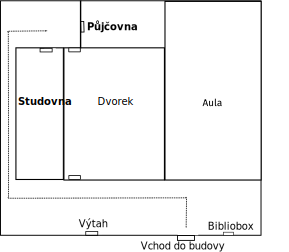
\includegraphics[width=\textwidth]{svgplanek.pdf}}
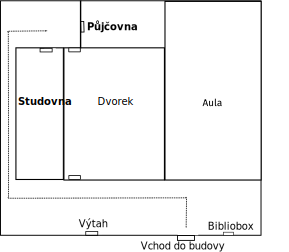
\includegraphics[width=\textwidth]{svgplanek.pdf}

\newpage
\section{Otevírací doba}

\noindent\smallsection{Půjčovna}

\ifdefined\HCode
\begin{tabular}{lllll}
  Po      & ~ & 8.00 &--& 16.00\\
  Út--pá  & ~ & 8.00 &--& 17.00
\end{tabular}

\else
Po 8.00 -- 16.00

Út 8.00 -- 17.00

St 8.00 -- 17.00

Čt 8.00 -- 17.00

Pá 8.00 -- 17.00
\fi

% \noindent\smallsection{Dočasná studovna}

% XXX

\newpage
\section{Kontakty}

\begin{tabular}{@{}ll@{}}
  E-mail:& \url{knihovna@pedf.cuni.cz}\\

  Půjčovna & 221~900~148\\

  % Studovna:& 221~900~178\\
  Studenti se SP:& 221~900~122\\
  Facebook & \url{@knihovnapedfpraha}\\
  Instagram & \url{@knihovnapedfpraha}
\end{tabular}

\subsection{Odkazy}

\begin{tabular}{@{}ll@{}}
  Knihovna PedF UK& \url{knihovna.pedf.cuni.cz} \\

  Centrální katalog UK& \url{ckis.cuni.cz} \\

  Centrální autentizační služba& \url{cas.cuni.cz} \\

  Portál elektronických zdrojů& \url{pez.cuni.cz} \\

  Vyhledávač UKAŽ & \url{ukaz.cuni.cz} \\

  Citace PRO & \url{citace.com/citace-pro} \\

  Ústřední knihovna UK & \url{knihovna.cuni.cz} \\

  IPSC UK & \url{ipc.cuni.cz} 
\end{tabular}
